\subsection{Determinação do volume e da densidade de um sólido com
uma balança}

O segundo experimento consiste em determinar o Volume de um sólido a partir da medida do Empuxo sofrido pelo objeto quando mergulhado em um líquido de densidade conhecida - nesse caso o líquido é a água. Para isso, será utilizado um sistema com uma balança que sofre a ação de uma “Força Normal”(N), que pode ser representado conforme a Imagem a seguir:

\begin{figure}[H]
    \centering
    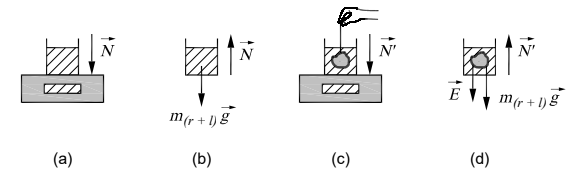
\includegraphics[scale=0.8]{images/Experimento2.png}
    \caption{Representação do experimento realizado em um sistema de balança que sofre a ação de uma força normal (N).}
\end{figure}

Com base na imagem, primeiramente determina-se a massa do recipiente com o líquido que será utilizado para submergir o corpo (a). Como o conjunto formado pelo recipiente e o líquido está em equilíbrio ($\sum$F=0), tem-se que a força normal (N), exercida pela superfície da balança perpendicularmente à parede do recipiente, é igual à força Peso (P) do sistema recipiente-líquido. Dessa forma, realizando as devidas manipulações matemáticas, tem-se que a massa do recipiente-líquido é igual a seguinte expressão:

\[ N = P \]
\[ N = m_{r+l} \cdot g \]
\[\therefore m_{r+l} = \frac{N}{g} \]

Entretanto, como está sendo utilizado uma balança digital, pode-se simplificar a obtenção da massa do sistema recipiente-líquido pela simples leitura do valor registrado na balança.

\begin{figure}[H]
    \centering
    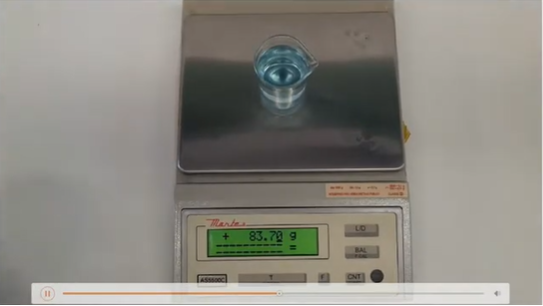
\includegraphics[scale=0.8]{images/Experimento2.2.png}
    \caption{Leitura da balança após incluir um recipiente com água.}
\end{figure}

Após isso, mergulha-se o corpo cujo volume se deseja determinar, segurando-o por um fio e tomando os devidos cuidados para que ele fique totalmente submerso no líquido e não toque nas laterais ou no fundo do recipiente (c). De forma análoga, a massa do sistema após adicionar o objeto submerso pode ser determinado por uma expressão que iguala a Força Normal (N’) à Força Peso (P’):

\[ N' = P' \]
\[ N' = m'_{r+l} \cdot g \]
\[\therefore m'_{r+l} = \frac{N'}{g} \]

Como também foi utilizado uma balança para essa etapa, também pode-se simplificar a obtenção do sistema após a adição do objeto pela simples leitura do valor registrado na balança.

\begin{figure}[H]
    \centering
    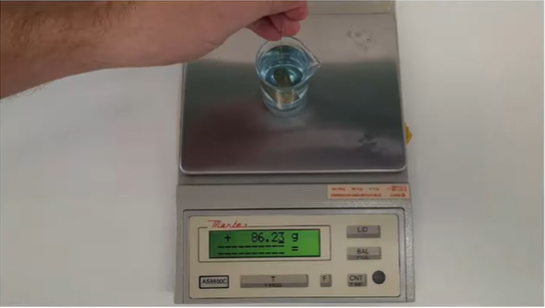
\includegraphics[scale=0.8]{images/Experimento2.1.png}
    \caption{Leitura da balança após incluir um sólido de volume desconhecido no recipiente com água.}
\end{figure}

Através do diagrama de forças do recipiente, com o líquido na situação em que o corpo está submerso, obtém-se as seguintes expressões:

\[ E = N' - m_{r+l} \cdot g \]
\[ \rho_1 \cdot V_s \cdot g = (m'_{r+l} - m_{r+l}) \cdot g \]
\[\therefore V_s = \frac{(m'_{r+l} - m_{r+l})}{\rho_1} \]

Como o líquido em questão no qual o sólido foi submerso é a água, cuja densidade é igual a $\rho_{agua}$ = 1,0 g/c$m^3$, a expressão acima pode ser sintetizada pela simples diferença entre as duas leituras da balança, ou seja, o Volume do sólido submerso ($V_s$) é igual a:

\[ V_s = m'_{r+l} - m_{r+l} \]

Depois de calculado o volume, será determinado a densidade desse sólido submerso ($\rho_{solido}$). Para isso, será determinado a massa do sólido diretamente pela leitura na balança. 

\begin{figure}[H]
    \centering
    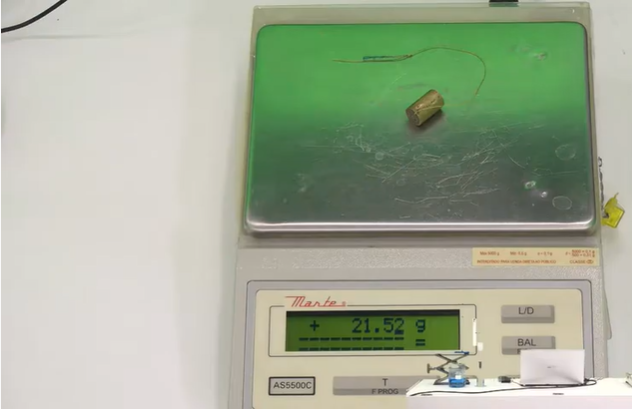
\includegraphics[scale=0.8]{images/Experimento2.3.png}
    \caption{ Leitura da balança após incluir o sólido.}
\end{figure}

Com esse valor e com o volume do sólido ($V_s$) calculado na etapa anterior, será determinado a Densidade do sólido pela seguinte expressão:

\[\rho_{solido} = \frac{m_{solido}}{V_s} \]

Após o cálculo, será feito a comparação da densidade obtida com o valor tabelado para, então, determinar de que material é feito o sólido.

